\newcommand{\SU}{\textit{Speed Up }}
\section{Principios fundamentales}

\subsection{Ejercicio resuelto: [1.2 $3^{ed}$ CAAQA]}
Se considera realizar una mejora a una máquina agregando hardware vectorial. Cuando un cálculo de modo vectorial se ejecuta en este hardware, este se realiza 10 veces más rápido que en modo de ejecución normal. Llamamos al porcentaje de tiempo que se puede utilizar este modo vectorial como porcentaje de vectorización.



Antes de resolver el ejercicio, planteamos el escenario mediante un diagrama:

%TODO Usar un include
\tikzset{every picture/.style={line width=0.75pt}} %set default line width to 0.75pt

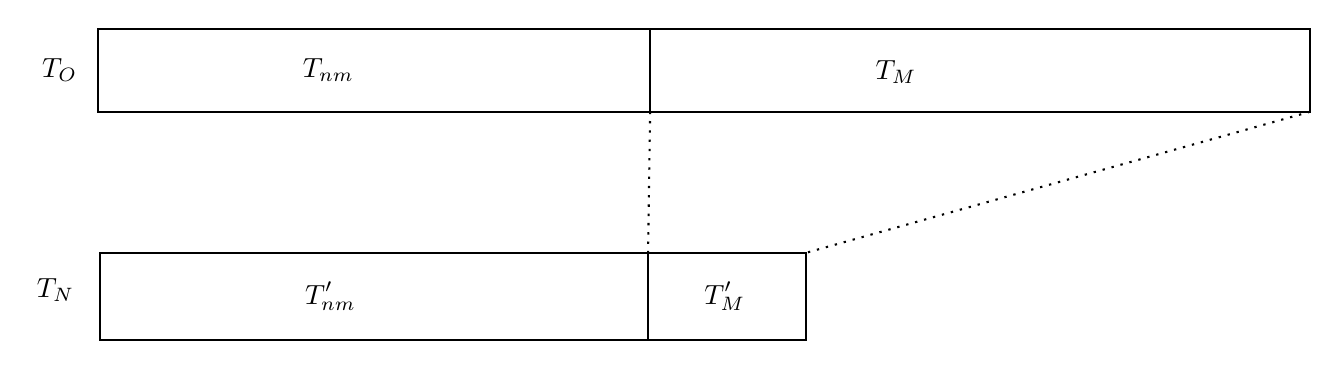
\begin{tikzpicture}[x=0.75pt,y=0.75pt,yscale=-1,xscale=1]
%uncomment if require: \path (0,300); %set diagram left start at 0, and has height of 300

%Shape: Rectangle [id:dp41842097652442645]
\draw   (39.5,21) -- (305.5,21) -- (305.5,61) -- (39.5,61) -- cycle ;
%Shape: Rectangle [id:dp8871764374832227]
\draw   (40.5,129) -- (304.5,129) -- (304.5,171) -- (40.5,171) -- cycle ;
%Shape: Rectangle [id:dp9269566177848496]
\draw   (305.5,21) -- (623.5,21) -- (623.5,61) -- (305.5,61) -- cycle ;
%Shape: Rectangle [id:dp3092576452949021]
\draw   (304.5,129) -- (380.5,129) -- (380.5,171) -- (304.5,171) -- cycle ;
%Straight Lines [id:da06697919884510961]
\draw  [dash pattern={on 0.84pt off 2.51pt}]  (305.5,61) -- (304.5,129) ;


%Straight Lines [id:da4571003142911374]
\draw  [dash pattern={on 0.84pt off 2.51pt}]  (623.5,61) -- (380.5,129) ;

% Text Node
\draw (21,41) node  [align=left] {$\displaystyle T_{O}$};
% Text Node
\draw (19,147) node  [align=left] {$\displaystyle T_{N}$};
% Text Node
\draw (424,42) node  [align=left] {$\displaystyle T_{M}$};
% Text Node
\draw (341.5,150) node  [align=left] {$\displaystyle T'_{M}$};
% Text Node
\draw (120,145) node  [align=left] {$ $};
% Text Node
\draw (151.5,150) node  [align=left] {$\displaystyle T'_{nm}$};
% Text Node
\draw (150.5,41) node  [align=left] {$\displaystyle T_{nm}$};

\end{tikzpicture}

\begin{enumerate}
 \item Realizar un gráfico que represente el \SU en función del como porcentaje de vectorización. Nombrar al \textit{eje y} como \SU Global ($SU_g$) y al \textit{eje x} como Porcentaje de Vectorización.

 Partiendo de la Ley de Amdahl, así como los datos del enunciado, tenemos que $$ SU_g = \frac{1}{(1-f) + \frac{f}{10}} = \frac{1}{1 - 0,9 \times f}$$
 Sabemos también que $ f \in [0, 1] $. Podemos calcular el valor de \SU en los extremos:
 \begin{itemize}
 \item Si no es posible aplicar la mejora, $f = 0 \implies SU_g = 1$
 \item Si la mejora es aplicable a todo el tiempo de ejecución, $ f = 1 \implies SU_g = SU_L = 10 $
 \end{itemize}

 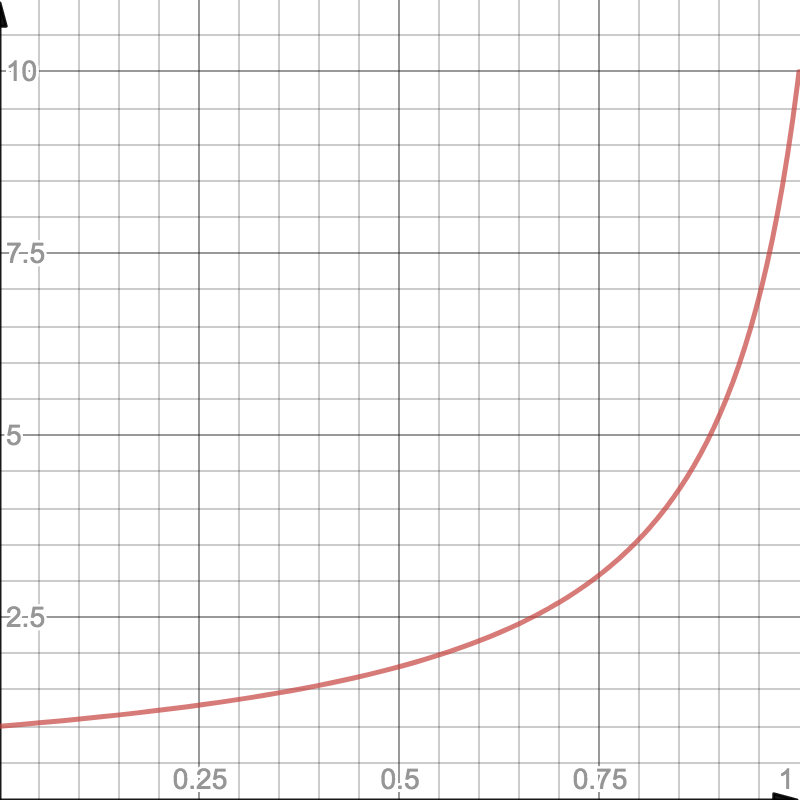
\includegraphics[scale=0.5]{gfx/amdahl_resuelto_1.png}
 
 \item ¿Qué porcentaje de vectorización en necesaria para alcanzar un \SU global de 2?

 Utilizando la ley de Amdahl podemos despejar $f$

 $$ 2 = \frac{1}{1 - 0,9 \times f}$$
 $$ f  = \sfrac{5}{9} $$
 
 \item ¿Qué porcentaje de tiempo se emplea en modo vectorización cuando se alcanza un \SU global de 2?

 Es importante entender que esta pregunta no es igual a la anterior. El escenario para este punto nos plantea en el momento en el que 
 la optimización ya se encuentra en ejecución.

 Partiendo de la definición de Speed Up, tenemos que 

 $$ SU_g = \frac{T_O}{T_N} = 2 \implies f = \sfrac{5}{9} $$

 $$ SU_L = \frac{T_m}{T'_m} = 10,\quad siendo \quad T_m = T_O \times f = \sfrac{5}{9}T_O $$

 El ejercicio nos pide calcular $ f' = \sfrac{T'_m}{T_N} $. Reemplazando se puede determinar que
 
 $$ T'_{nm} = T_{nm} = \sfrac{4}{9} \times T_O $$
 $$ T'_m =  \sfrac{T_m}{10} $$ 
 $$ T_N = T'_{m} + T'_{nm} $$
 $$ T_{nm} = T'_{nm} $$ 
 
 $ f' = \frac{\frac{5}{90}}{\frac{5}{90} + \frac{4}{9}} $
 
 \item ¿Qué porcentaje de vectorización es necesaria para alcanzar la mitad del máximo \SU posible al usar el modo de vectorización?

 A partir de la Ley de Amdahl y el análisis realizado en el primer punto sabemos qué $SU_{max} = 10$, por lo que solo resta resolver

 $$ \frac{1}{5} = 1 - 0,9 \times f $$
 $$ f = \frac{8}{9} $$ 
 
 \item Ahora suponga que se realizó una medición y se determinó que el porcentaje de vectorización para ciertos programas es del 70\%. El grupo de diseño de hardware dice que pueden duplicar el \SU del hardware de vectorización pero con una inversión significante en lo que respecta. Entonces nos preguntamos si el equipo de compiladores podrían incrementar el uso del modo vectorizado (relativo al uso actual) para lograr la misma performance obtenida al aumentar al doble el \SU por hardware. ¿Qué inversión recomendaría?  

\end{enumerate}


\subsection{}
Demostrar que 

						 $$ SU = \frac {1} {(1-f) + \frac {f}{SU_l}} $$


Donde $f$ es la fracción de tiempo a mejorar, y $SU_l$ es la mejora local.

\subsection{}

Un procesador de 300 Mhz ejecuta un programa que presenta los siguientes tipos de instrucciones:

\begin{table}[h!]
\begin{tabular}{|l|c|c|}
\hline
 Tipo de instrucción & Frecuencia (\%)  &  Ciclos  \\ \hline
 Aritmético-Lógica & 40  &  1  \\ \hline
 Carga & 20 & 1 \\ \hline
 Almacenamiento & 10  & 2  \\ \hline
 Saltos & 20  & 3 \\ \hline
 Punto Flotante & 10 & 5  \\ \hline
\end{tabular}
\end{table}

\begin{enumerate}[label=\alph*)]
 \item Calcular las tasas de CPI y MIPS, para el programa completo.
 \item Suponga que una optimización elimina un 30 \% de las instrucciones aritmético-lógicas (o sea, 12 \% del total de instrucciones A-L), 30 \% de instrucciones load y 20 \% de punto flotante. ¿Cuál es el speedup alcanzado?
 \item Recalcular las tasas de CPI y MIPS para el programa completo. Explicar las diferencias respecto al punto (a).
\end{enumerate}

\subsection{}
Se proponen 3 mejoras para una nueva arquitectura con los siguientes Speedups:
\begin{itemize}
\item Speedup1 = 30
\item Speedup2 = 20
\item Speedup3 = 10
\end{itemize}

Sólo una mejora es aplicable en cada momento (no se pueden solapar).

\begin{enumerate}[label=\alph*)]
 \item Si las mejoras 1 y 2 se pueden usar un 30 \% del tiempo, ¿qué fracción del tiempo se debe usar la mejora 3 para lograr un speedup global de 10?
 \item Asumir que la distribución del uso de las mejoras es del 30 \%, 30 \% y 20 para las mejoras 1, 2 y 3 respectivamente. Asumir que las 3 mejoras están en uso. ¿Qué fracción del tiempo mejorado no tiene una mejora en uso?
 \item Asumir que para un benchmark la fracción del uso de las mejoras es del 15 \% para 1 y 2 y del 70 \% para la mejora 3. Se quiere maximizar la performance. Si sólo una mejora puede ser aplicada, ¿cuál debería ser elegida? Si 2 mejoras pueden ser aplicadas, ¿cuales deberían ser elegidas?
\end{enumerate}

\subsection{}
Se dispone de un benchmark que contiene $195,578$ instrucciones de punto flotante.
	
Dicho Benchmark fue ejecutado en un procesador embebido luego de haber sido compilado con las optimizaciones activadas. El procesador embebido está basado en un procesador RISC que incluye unidades de punto flotante, pero el procesador embebido no dispone de ellas por distintas razones. El compilador permite calcular las operaciones de punto flotante mediante unidades punto flotante o mediante rutinas de software, dependiendo en las opciones utilizadas.
	
El benchmark se ejecutó en $1,08$ segundos en el procesador RISC, mientras que tomó $13.6$ segundos en la versión embebida. Asumir que el CPI del procesador RISC es $10$, mientras que el CPI del procesador embebido es $6$.
	
\begin{enumerate}[label=\alph*)]
\item Para ambos procesadores, ¿cuántas instrucciones fueron ejecutadas?
\item Para ambos procesadores, ¿cuál es el valor de la tasa de MIPS?
\item En promedio, ¿cuántas instrucciones enteras son necesarias para ejecutar una operación de punto flotante en software?
\end{enumerate}
	
Responder considerando que el benchmark puede estar conformado por 
	
\begin{itemize}
    \item Un $100\%$ de instrucciones de punto flotante.
    \item Instrucciones de punto flotante y enteras.
\end{itemize}


\subsection{[1.3 $3^{ed}$ CAAQA]}
Se realiza una mejora a una computadora a un dado modo de ejecución por un factor de 10. Esta mejora es utilizada el 50\% del tiempo, medido como un porcentaje del tiempo de ejecución cuando la mejora está siendo utilizada. Recordar que no se puede aplicar directamente este 50\% en la Ley de Amdahl para para calcular el speedup.

\begin{enumerate}
 \item ¿Cuál es el speedup global que se alcanza con esta mejora?
 \item ¿Qué porcentaje del tiempo original es empleada esta mejora?
\end{enumerate}


\subsection{[1.6 $3^{ed}$ CAAQA]}
Un benchmark muy conocido para enteros es Dhrystone. La computadora A realiza D A ejecuciones del benchmark por segundo y realiza millones de instrucciones por segundo (MIPS A). En la computadora B se ejecuta el mismo benchmark obteniendo sus propias métricas.

\begin{enumerate}
 \item ¿Cuál es el problema en calcular la tasa de MIPS de la computadora B como $MIPS_B = MIPS_A \times (D_B / D_A )$?
\end{enumerate}



\subsection{[1.17 $3^{ed}$ CAAQA]}
Una empresa tiene un benchmark que es considerado representativo para sus aplicaciones típicas. Se está considerando un procesador embebido para realizar las tareas pero no cuenta con una unidad de punto flotante y se deben emular por una secuencia de instrucciones de enteros. Este procesador tiene una tasa de 120 MIPS en el benchmark.

Un vendedor ofrece un coprocesador para mejorar la performance. Este coprocesador ejecuta cada instrucción de punto flotante por hardware. Cuando se combina el procesador y el coprocesador resulta una tasa de MIPS de 80 en el mismo benchmark.

Sea:

\begin{itemize}
 \item I: Número de instrucciones de enteros ejecutadas en el benchmark.
 \item F: Número de instrucciones de punto flotante ejecutadas en el benchmark.
 \item Y: Número de instrucciones de entero para emular las instrucciones de punto flotante.
 \item W: Tiempo de ejecución del benchmark en el procesador solo.
 \item B: Tiempo de ejecución del benchmark en la combinación procesador/coprocesador.
\end{itemize}

\begin{enumerate}
 \item Escribir una expresión para calcular la tasa de MIPS en cada configuración utilizando los símbolos anteriores.
 \item Para la configuración sin coprocesador, se obtuvo $F = 8 \times 10^6$, $Y = 50$ y $W = 4$ segundos. Determinar I.
 \item ¿Cuál es el valor de B?
 \item ¿Cuál es la tasa de MFLOPS para el sistema con coprocesador?
 \item Un colega quiere comprar el coprocesador a pesar que tiene una tasa de MIPS inferior cuando se lo utiliza en comparación con el procesador sólo. ¿Tiene razón? Justificar la respuesta.
\end{enumerate}


